%\documentclass{article}
\documentclass[a4paper]{article}
\usepackage[a4paper, total={6in, 8in}]{geometry}
%\usepackage[showframe]{geometry}
%\usepackage{layout}
%\setlength{\voffset}{-0.75in}
%\setlength{\headsep}{5pt}

\sloppy

\usepackage{graphicx}
\graphicspath{ {images/} }

\usepackage{amsmath}
\usepackage[makeroom]{cancel}

\usepackage{hyperref}

\title{Maximum Speed-Up}
\author{San Kho Lin}
\date{}

\begin{document}

%\maketitle

\noindent
{\huge Maximum Speed-Up}

%\section{Introduction}
%A study note for the approaches to show maximum speed-up.

\section{Amdahl's Law}
\subsection{Proof}
In general case the speed-up of the parallel computation is:

\begin{center}
{\Large $S(N) = \frac{T(1)}{T(N)}$}
\end{center}
\verb|T(1)| = the execution time of the sequential computation
\\
\verb|T(N)| = the execution time when N parallel computations
\\
\\
\noindent
Amdahl's Law gives the potential speed-up of a parallel computation; it
states that the portion of the computation that cannot be parallelized determines the overall speed-up. If $\alpha$ (alpha) is the fraction of running time a sequential program spends on \textbf{non-parallelizable} segments of the computation, then for a very large N, the speed-up is limited to:

\begin{center}
{\Large $S = \frac{1}{\alpha}$}
\end{center}

\noindent
$\sigma$ = Let call \textit{Sigma} the sequential part
\\
$\pi$ = Let call \textit{Pi} the parallel part
\\
\\
Then we get:
\\
\\
total time taken for 1 processor = sequential part + parallel part
\begin{center}
{\Large $T(1) =  \sigma + \pi$}
\end{center}
total time taken for parallel N processes = sequential part + parallel part divided by N
\\
\begin{center}
{\Large $T(N) = \sigma + \frac{\pi}{N}$}
\end{center}

\begin{figure}[h]
\label{fig:ap1}
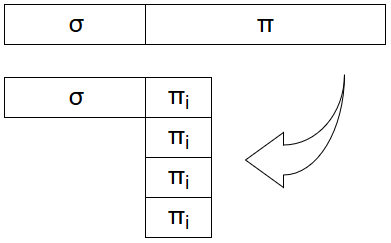
\includegraphics[scale=0.6]{serial_parallel_parts.png}
\centering
%\caption{Decomposition of Computation}
%\centering
\end{figure}

\noindent
Whereas {\Large $\pi_{i} = \frac{\pi}{N}$}

\pagebreak

\noindent
Then
\begin{large}
\begin{equation}
S(N) = \frac{T(1)}{T(N)} = \frac{\sigma + \pi}{\sigma + \frac{\pi}{N}} =  \frac{\bcancel{\sigma} (1 + \frac{\pi}{\sigma})}{\bcancel{\sigma} (1 + \frac{\pi}{\sigma} + \frac{1}{N} )} = \frac{1 + \frac{\pi}{\sigma}}{1 + \frac{\pi}{\sigma} + \frac{1}{N}}
\end{equation}
\end{large}
\\
\\
\noindent
And since $\alpha$ is the fraction of running time a sequential program spends on \textbf{non-parallelizable} segments of the computation, we get:

\begin{large}
\begin{align*}
\alpha &= \frac{\sigma}{\sigma + \pi} \\
\sigma + \pi &= \frac{\sigma}{\alpha} \\
\pi &= \frac{\sigma}{\alpha} - \sigma \\
\pi &= \sigma (\frac{1}{\alpha} - 1) \\
\frac{\pi}{\sigma} &= \frac{1}{\alpha} - 1 \\
\frac{\pi}{\sigma} &= \frac{1 - \alpha}{\alpha}
\end{align*}
\end{large}

Let {\large $\frac{\pi}{\sigma} = \frac{1 - \alpha}{\alpha}$} substitute into equation (1), we get:

\begin{Large}
\begin{align*}
S &= \frac{1 + \frac{1 - \alpha}{\alpha}}{1 + \frac{1 - \alpha}{\alpha} \cdot \frac{1}{N}} = \frac{1 + \frac{1 - \alpha}{\alpha}}{1 + \frac{1 - \alpha}{N\alpha}} = \frac{\frac{\cancel{\alpha} + 1 - \cancel{\alpha}}{\alpha}}{\frac{N\alpha + 1 - \alpha}{N\alpha}} \\
&= \frac{1}{\cancel{\alpha}} \times \frac{N\cancel{\alpha}}{N\alpha + 1 - \alpha} = \frac{N}{N\alpha + 1 - \alpha} \\
&= \frac{\cancel{N}}{\cancel{N}(\alpha + \frac{1}{N} - \frac{\alpha}{N})} = \frac{1}{\alpha + \frac{1}{N} - \frac{\alpha}{N}} \\
&= \frac{1}{\alpha + \frac{1 - \alpha}{N}} \\
&\approx \frac{1}{\alpha} \text{ for large N}
\end{align*}
\end{Large}

%\noindent
%Therefore, we get $\approx \frac{1}{\alpha}$ theoretical assumption for very large N.
%\\
%\\

\pagebreak

\subsection{Another Way}
Alternatively, we may also express a speed-up factor:

\[
S(p) = \frac{\text{execution time using one processor}}{\text{execution time using p processors}} = \frac{T(1)}{T(p)} = \frac{t_s}{t_p}
\]

\noindent
$p$ = the number of processors
\\
$t_s$ = the sequential execution time
\\
$t_p$ = the parallel execution time
\\
\\
\noindent
Let $f$ be the fraction of the computation that cannot be divided into concurrent tasks, and no overhead is incurred when the computation is divided into concurrent parts, the time to perform the computation with $p$ processors is given by:

\begin{center}
{\Large $ft_s + \frac{(1 - f)t_s}{p}$}
\end{center}

\begin{figure}[h]
\label{fig:ap2}
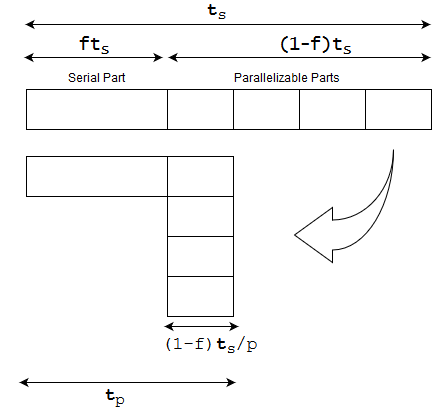
\includegraphics[scale=0.9]{alternate_representation.png}
\centering
%\caption{Parallelizing sequential problem -- Amdahl's Law}
%\centering
\end{figure}

\pagebreak

\noindent
The illustration is the case with a single serial part at the beginning of the computation, but the serial part could be distributed throughout the computation. Hence, the speed-up factor is given by:

\begin{Large}
\begin{align*}
S(p) &= \frac{t_s}{ft_s + \frac{(1 - f)t_s}{p}} 
= \frac{\bcancel{t_s}}{\bcancel{t_s}(f + \frac{1 - f}{p})} \\
&= \frac{1}{\frac{fp + 1 - f}{p}} 
= \frac{p}{fp + 1 - f} \\
&= \frac{p}{1 + (fp - f)} 
= \frac{p}{1 + (p - 1)f} \\
&\approx \frac{1}{f} \text{ for large p}
\end{align*}
\end{Large}

\noindent
With an infinite number of processors, the maximum speed-up is limited to {\Large $\frac{1}{f}$} i.e.,
\begin{center}
{\Large $S(p)_{p \to \infty} = \frac{1}{f}$}
\end{center}

\subsection{Applied Amdahl's Law}

\noindent
\textbf{Case 1:} If 95\% of the program can be parallelized, the theoretical maximum speed-up using parallel computing would be 20x, no matter how many processors are used: 
\begin{center}
{\large $S = \frac{1}{\alpha} = \frac{1}{100\% - 95\%} = \frac{1}{1 - 0.95} = \frac{1}{0.05} = 20$}
\end{center}
i.e. if the non-parallelisable part takes 1 hour, then no matter how many CPU cores you throw at it, it won't complete in less than 1 hour. With only 5\% of the computation being serial, the maximum speed-up is 20, irrespective of the number of processors.
\\
\\
\noindent
\textbf{Case 2:} Consider a case when the fraction of the problem that cannot be parallelized is a function of the problem size, $f(n)$. Then the speed-up is {\large $\frac{1}{f(n)}$} for large number of processors.

\noindent
e.g., consider sorting where the elements to be sorted are read sequentially from disk. For a problem of size $n$, the average sequential run time for best sorting algorithm is $\Theta(n\log{}n)$. If the sorting computations can be completely parallelized then the fraction that cannot be parallelized is:

\begin{center}
{\large $f(n) = \Theta(\frac{n}{n\log{}n}) = \Theta(\frac{1}{\log{}n})$}
\end{center}

\noindent
Therefore, for a large number of processors the speed-up is limited to $\log{}n$ which probably reading elements from the disk sequentially.

\subsection{Over Simplifications}
Consider a program that executes a single loop, where all iterations can be computed independently, i.e. code can be parallelized. By splitting the loop into several parts, e.g. one loop iteration per processor, each processor now has to deal with loop overheads such as calculation of bounds, test for loop completion etc. This overhead is replicated as many times as there are processors. In effect, loop overhead acts as a further (serial) overhead in running the code. Also getting data to/from many
processor overheads? 
\\
\\
In a nutshell Amdahl's Law greatly simplifies the real world!
\\
\\
Amdahl's law applies to a fixed problem size; in this case the amount of work assigned to each one of
the parallel processes decreases when the number of processes increases, and this affects the efficiency of the parallel execution.
\noindent
Since it assumes a fixed problem size – sometimes it can't predict length of time required for jobs,
-  e.g. state space exploration or differential equations that don't solve...

\section{Gustafson-Barsis's Law}
\subsection{Proof}
Also shorten as Gustafson's Law. When the problem size is allowed to change, Gustafson's Law gives the scaled speed-up with N parallel processes as:
\begin{center}
$S(N) = N - \alpha(N - 1)$
\end{center}
\noindent
$\sigma$ = the sequential time \\
$\pi$ = the fixed parallel time per process \\
The sequential execution time: $T(1) = \sigma + N\pi$ \\
The parallel execution time with N parallel processes: $T(N) = \sigma + \pi$ 

\begin{large}
\begin{align}
S(N) = \frac{T(1)}{T(N)} = \frac{\sigma + N\pi}{\sigma + \pi} = \frac{\sigma}{\sigma + \pi} + \frac{N\pi}{\sigma + \pi} = \frac{\sigma}{\sigma + \pi} +  N \frac{\pi}{\sigma + \pi}
\end{align}
\end{large}

\noindent
And since $\alpha$ is the fraction of running time a sequential program spends on \textbf{non-parallelizable} segments of the computation, we get:
\begin{large}
\begin{align*}
\alpha &= \frac{\sigma}{\sigma + \pi} \\
1 - \alpha &= 1 - \frac{\sigma}{\sigma + \pi} \\
1 - \alpha &= \frac{\bcancel{\sigma} + \pi - \bcancel{\sigma}}{\sigma + \pi}
\end{align*}
\end{large}

Let {\large $\frac{\sigma}{\sigma + \pi} = \alpha$} and {\large $\frac{\pi}{\sigma + \pi} = 1 - \alpha$} substitute into equation (2), we get:

\begin{large}
\begin{align*}
S(N) &= \alpha + N (1 - \alpha) = \alpha + N - N\alpha  \\
&= N + \alpha - N\alpha = N - \alpha(N - 1)
\end{align*}
\end{large}

\noindent
Both Amdahl's Law and the scaled speed-up assume that all processes are assigned the same amount of work. The scaled speed-up assumes that the amount of work assigned to each process is the same, regardless of the problem size. Then, to maintain the same execution time, the number of parallel processes must increase with the problem size.
\\
\\
\noindent
The scaled speed-up captures the essence of efficiency, namely that the limitations of the sequential part of a code can be balanced by increasing the problem size.
\\
\\
\noindent
Speed up S using N processes is given as a linear formula dependent on the number of processes and the fraction of time to run sequential parts. Gustafson's Law proposes that programmers tend to set the size of problems to use the available equipment to solve problems within a practical fixed time. Faster (more parallel) equipment available, larger problems can be solved in the same time.

\subsection{Another Way}
Alternatively, here is an another way to express Gustafson law that correspond to section 1.2.

\begin{itemize}
\item Gustafson presented an argument based upon scalability concepts to show that Amdahl's law was not as significant as first supposed in determining the potential speed-up limits. Gustafson attributed formulating the idea into an equation to \emph{E.Barsis}.

\item Gustafson makes the observation that in practice a larger multiprocessors usually allows a larger problem to be undertaken in a reasonable execution time. Hence in practice, the problem size selected frequently depends of the number of available processors. Rather than assume that the problem size is fixed, it is just as valid to assume that the parallel execution time is fixed. 

\item As the system size is increased ($p$ increased), the problem size is increased to maintain constant parallel-execution time. In increasing the problem size, Gustafson also makes the case that the serial section of the code is normally fixed and does not increase with the problem size.

\item Using the constant parallel-execution time constraint, the resulting speed-up factor will be numerically different from Amdahl's speed-up factor and is called a \textbf{scaled speed-up factor} (i.e, the speed-up factor when the problem is scaled). For Gustafson's scaled speed-up factor, the parallel execution time, $t_p$, is constant rather than the serial execution time, $t_s$, in Amdahl's law.

\item For the derivation of Gustafson's law, we shall use the same terms as for deriving Amdahl's law, but it is necessary to separate out the serial and parallelizable sections of the sequential execution time, $t_s$, into $ft_s + (1 - f)t_s$ as the serial section $ft_s$ is a constant. For algebraic convenience, let the parallel execution time, $t_p = ft_s + (1 - f) t_s/p = 1$. Then, with a little algebraic manipulation, the serial execution time, $t_s$, becomes $ft_s + (1 - f)t_s = p + (1 - p)ft_s$. The scaled speed-up factor then becomes (which is called Gustafson's law)

\begin{large}
\begin{align*}
S_s(p) = \frac{ft_s + (1 - f)t_s}{ft_s + \frac{(1 - f)t_s}{p}} = \frac{p + (1 - p)ft_s}{1} = p + (1 - p)ft_s
\end{align*}
\end{large}

\item There are two assumptions in this equation: the parallel execution time is constant, and the part that must be executed sequentially, $ft_s$, is also constant and not a function of $p$. 
\end{itemize}


%Gustafson's observation here is that the scaled speed-up factor is a line of negative slope(1 - p) rather than the rapid reduction previously illustrated in 1.3(b). 
\noindent
For example, suppose we had a serial section of 5\% and 20 processors; the speed-up is $0.05 + 0.95(20) = 19.05$ according to the formula instead of $10.26$ according to Amdahl's law. (Note, however, the different assumptions.)
\\
\\
\noindent
Apart from constant problem size scaling (Amdahl's assumption) and time-constrained scaling (Gustafson's assumption), scaling could be memory-constrained scaling. In memory-constrained scaling, the problem is scaled to fit in the available memory. As the number of processors grows, normally the memory grows in proportion. This form can lead to significant increases in the execution time.


%---


\begin{thebibliography}{9}
\bibitem{dan} 
Dan C. Marinescu. 
\textit{Cloud Computing Theory and Practice}. 
Elsevier, ISBN: 978-0-12404-627-6, 2013.

\bibitem{wilkin} 
Barry Wilkinson and Michael Allen. 
\textit{Parallel Programming, Techniques and Applications Using Networked Workstations and Parallel Computers 2nd Edition}. 
Prentice Hall, ISBN: 0-13-140563-2, 2005. 
\end{thebibliography}

\noindent
Prepared by \textit{San Kho Lin} and available at \url{https://github.com/victorskl/speedup}


\end{document}